\documentclass[tikz,border=3mm]{standalone}
\usepackage[T1]{fontenc}
\usepackage{helvet}
\renewcommand{\familydefault}{\sfdefault}
\usepackage{amsmath,amssymb}
\usepackage{tikz}
\usetikzlibrary{shapes.geometric, positioning, arrows.meta, calc}

\begin{document}
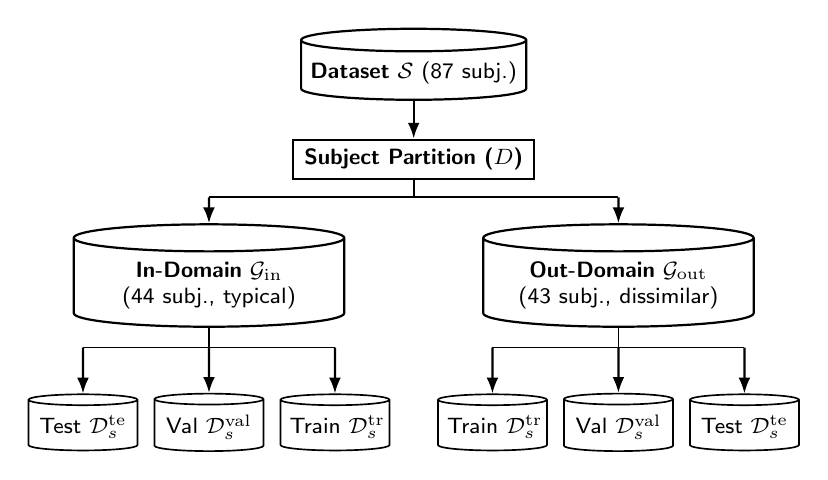
\begin{tikzpicture}[
  every node/.style={font=\sffamily\footnotesize},
  >=Latex,
  db/.style={draw, thick, cylinder, cylinder uses custom fill,
    cylinder body fill=white, shape border rotate=90, aspect=0.10,
    minimum width=2.6cm, minimum height=0.7cm, align=center,
    font=\sffamily\footnotesize},
  dbsm/.style={draw, semithick, cylinder, cylinder uses custom fill,
    cylinder body fill=white, shape border rotate=90, aspect=0.10,
    minimum width=1.35cm, minimum height=0.5cm, text width=1.15cm,
    align=center, font=\sffamily\footnotesize},
  pbox/.style={draw, thick, align=center, fill=white,
    minimum height=0.5cm, inner xsep=4pt, inner ysep=2pt,
    font=\sffamily\footnotesize},
  arr/.style={-{Latex[length=2mm, width=1.5mm]}, thick},
]

%% ---- Dataset ----
\node[db] (dataset) at (0,0)
  {\textbf{Dataset}~$\mathcal{S}$ (87 subj.)};

%% ---- D: Subject Partition ----
\node[pbox] (dsplit) at (0,-1.10)
  {\textbf{Subject Partition ($D$)}};
\draw[arr] (dataset.south) -- (dsplit.north);

%% ---- In / Out groups ----
\node[db, text width=3.2cm] (src) at (-2.6,-2.7)
  {\textbf{In-Domain}~$\mathcal{G}_{\mathrm{in}}$\\(44 subj., typical)};
\node[db, text width=3.2cm] (tgt) at ( 2.6,-2.7)
  {\textbf{Out-Domain}~$\mathcal{G}_{\mathrm{out}}$\\(43 subj., dissimilar)};

\coordinate (forkMid) at ($(dsplit.south)!.4!(src.north)$);
\coordinate (forkC) at (0,0 |- forkMid);
\coordinate (forkL) at (-2.6,0 |- forkMid);
\coordinate (forkR) at ( 2.6,0 |- forkMid);
\draw[thick] (dsplit.south) -- (forkC);
\draw[thick] (forkL) -- (forkR);
\draw[arr] (forkL) -- (src.north);
\draw[arr] (forkR) -- (tgt.north);

%% ---- Per-subject 70/15/15 split (In-Domain side) ----
\node[dbsm] (test_s)  at (-4.2,-4.5) {Test~$\mathcal{D}_s^{\mathrm{te}}$};
\node[dbsm] (val_s)   at (-2.6,-4.5) {Val~$\mathcal{D}_s^{\mathrm{val}}$};
\node[dbsm] (train_s) at (-1.0,-4.5) {Train~$\mathcal{D}_s^{\mathrm{tr}}$};

\coordinate (forkS) at ($(src.south)!.30!(test_s.north)$);
\draw[semithick] (src.south) -- (-2.6,0 |- forkS);
\draw[semithick] (-4.2,0 |- forkS) -- (-1.0,0 |- forkS);
\draw[arr] (-4.2,0 |- forkS) -- (test_s.north);
\draw[arr] (-2.6,0 |- forkS) -- (val_s.north);
\draw[arr] (-1.0,0 |- forkS) -- (train_s.north);

%% ---- Per-subject 70/15/15 split (Out-Domain side) ----
\node[dbsm] (train_t) at (1.0,-4.5)  {Train~$\mathcal{D}_s^{\mathrm{tr}}$};
\node[dbsm] (val_t)   at (2.6,-4.5)  {Val~$\mathcal{D}_s^{\mathrm{val}}$};
\node[dbsm] (test_t)  at (4.2,-4.5)  {Test~$\mathcal{D}_s^{\mathrm{te}}$};

\coordinate (forkT) at ($(tgt.south)!.30!(test_t.north)$);
\draw[semithick] (tgt.south) -- (2.6,0 |- forkT);
\draw[semithick] (1.0,0 |- forkT) -- (4.2,0 |- forkT);
\draw[arr] (1.0,0 |- forkT) -- (train_t.north);
\draw[arr] (2.6,0 |- forkT) -- (val_t.north);
\draw[arr] (4.2,0 |- forkT) -- (test_t.north);

\end{tikzpicture}
\end{document}
